% 2005 年山东卷理科第 2 题：反函数图象 4 个选项 (A)~(D)
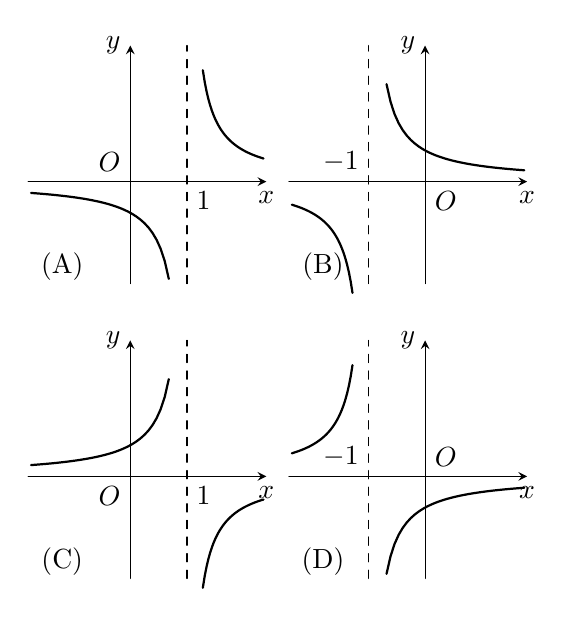
\begin{tikzpicture}[>=stealth,scale=0.72,line cap=round]
  % (A) 垂直渐近线 x = 1，双曲线递减分支
  \begin{scope}
    \draw[->] (-1.8,0)--(2.4,0) node[below] {$x$};
    \draw[->] (0,-1.8)--(0,2.4) node[left] {$y$};
    \node[above left] at (0,0) {$O$};
    \draw[dashed] (1,-1.8)--(1,2.4);
    \node[below right] at (1,0) {$1$};
    \draw[thick,domain=1.28:2.35,samples=35] plot (\x,{0.55/(\x-1)});
    \draw[thick,domain=-1.75:0.68,samples=35] plot (\x,{0.55/(\x-1)});
    \node at (-1.2,-1.5) {(A)};
  \end{scope}

  % (B) 垂直渐近线 x = -1，双曲线递减分支（正确选项）
  \begin{scope}[xshift=5.2cm]
    \draw[->] (-2.4,0)--(1.8,0) node[below] {$x$};
    \draw[->] (0,-1.8)--(0,2.4) node[left] {$y$};
    \node[below right] at (0,0) {$O$};
    \draw[dashed] (-1,-1.8)--(-1,2.4);
    \node[above left] at (-1,0) {$-1$};
    \draw[thick,domain=-0.68:1.75,samples=35] plot (\x,{0.55/(\x+1)});
    \draw[thick,domain=-2.35:-1.28,samples=35] plot (\x,{0.55/(\x+1)});
    \node at (-1.8,-1.5) {(B)};
  \end{scope}

  % (C) 垂直渐近线 x = 1，双曲线递增分支
  \begin{scope}[yshift=-5.2cm]
    \draw[->] (-1.8,0)--(2.4,0) node[below] {$x$};
    \draw[->] (0,-1.8)--(0,2.4) node[left] {$y$};
    \node[below left] at (0,0) {$O$};
    \draw[dashed] (1,-1.8)--(1,2.4);
    \node[below right] at (1,0) {$1$};
    \draw[thick,domain=1.28:2.35,samples=35] plot (\x,{-0.55/(\x-1)});
    \draw[thick,domain=-1.75:0.68,samples=35] plot (\x,{-0.55/(\x-1)});
    \node at (-1.2,-1.5) {(C)};
  \end{scope}

  % (D) 垂直渐近线 x = -1，双曲线递增分支
  \begin{scope}[xshift=5.2cm,yshift=-5.2cm]
    \draw[->] (-2.4,0)--(1.8,0) node[below] {$x$};
    \draw[->] (0,-1.8)--(0,2.4) node[left] {$y$};
    \node[above right] at (0,0) {$O$};
    \draw[dashed] (-1,-1.8)--(-1,2.4);
    \node[above left] at (-1,0) {$-1$};
    \draw[thick,domain=-0.68:1.75,samples=35] plot (\x,{-0.55/(\x+1)});
    \draw[thick,domain=-2.35:-1.28,samples=35] plot (\x,{-0.55/(\x+1)});
    \node at (-1.8,-1.5) {(D)};
  \end{scope}
\end{tikzpicture}